\begin{problem}{나무나무나 심어야지}{standard input}{standard output}{2 seconds}{1024 megabytes}

근성은 나무에 관심이 많다.  
비록 지금은 코딩을 하고 있지만, 그렇다고 나무에 대한 애정이 식은 것은 아니다.
어느 날 이진 트리를 가지고 놀던 근성은 이진 트리는 나무임에도 열매가 안 열린다는 사실을 깨닫고 큰 충격에 빠졌다. 
근성은 나무는 열매가 반드시 열려야 한다 생각하는 나무열매..(중략) 론을 밀고 있었기에 나무 열매가 열리는 트리 그래프를 만들었고 이에 "나무나무"라 이름 지었다.

나무나무의 특징은 다음과 같다.
\begin{enumerate}
\item 이 트리의 1번 정점은 뿌리를 의미한다. 이 트리는 뿌리로부터 위로 뻗어 나간다.
\item 1번 정점을 제외한 정점은 가지가 갈라지는 지점을 의미한다. 정점에는 가지가 연결될 수 있다. 단, 다른 가지에서 갈라진 가지가 정점에서 합쳐지지는 않는다.
\item 간선은 가지를 의미한다. 가지 양 끝에는 반드시 정점이 존재한다.
\item 정점에는 최대 1개의 열매가 열릴 수 있다.
\end{enumerate}

트리를 만든 후 무엇을 할 수 있을까 고민하던 중 아래와 같은 두 가지를 생각해 냈다!
\begin{itemize}
  \item \bf{1 i j w  (접목)} : 임의의 정점 i에 가지를 붙인다.
    \begin{itemize}
      \item 정점 i는 뿌리와 한 그래프에 속하는 정점이다.
      \item 가지 끝에는 정점이 항상 존재하기에 j번으로 번호를 붙인 정점이 가지 반대쪽에 같이 붙는다.
      \item 정점 j에는 w 무게의 열매가 달린다. 열매가 없다면 0이 주어진다.
      \item (1≤ i, j ≤ N + M; 0 ≤ w ≤ 500)
    \end{itemize}
  \item \bf{2 i (수확)} : 정점 i 위로 달린 열매를 모두 떨어트리려면 몇의 힘으로 흔들어야 할지 출력한다.
    \begin{itemize}
      \item 임의의 정점 i를 흔들면 해당 정점 위로 연결된 가지, 정점들이 모두 흔들린다.  
      \item a 무게를 가지는 열매는 a만큼의 힘으로 흔들어야 떨어진다.
      \item 흔들리는 열매가 여러 개면 그만큼 힘이 분산되기에 a 무게와 b 무게의 열매가 있다면 a + b의 힘으로 흔들어야 둘 다 떨어진다.
      \item (1≤ i ≤ N + M )
    \end{itemize}
\end{itemize}


열매는 떨어트려도 나무나무의 특수한 힘으로 다음 쿼리 이전에 자라난다.
쿼리에 주어지는 수는 모두 정수이고, 올바른 입력임을 보장한다. 또한 수확쿼리는 1회 이상 주어진다.


그런데 근성은 이 쿼리를 만들다 갑자기 동아리방에 가야 한다며 도망쳤다.
여러분이 대신 풀어주자

\InputFile
첫째 줄에 최초 정점의 수 N개, 쿼리의 수 M이 주어진다. 
최초의 정점에는 1~N 사이의 번호가 중복되지 않게 붙어있다. (2≤ N , M ≤ 100,000)

둘째 줄에 N개의 정점이 각각 몇 번 정점에서 나온 가지에 있는 것인지 주어진다.
1번은 뿌리이므로 -1이 주어진다.
모든 정점은 최종적으로 뿌리와 한 그래프에 속하지만, 입력 도중에는 속하지 않을 수 있다.

셋째 줄에 N개의 정점이 가지고 있는 열매의 무게가 주어진다. 0이라면 열매가 없는 것이고 뿌리는 열매를 가지지 않는다.

이후 넷째 줄부터 M개의 줄에 걸쳐 쿼리가 주어진다.

\OutputFile
수확 쿼리가 들어올 때 몇의 힘으로 흔들어야 할지 출력한다. 단, 흔들어야 할 힘이 0이라면 -1을 출력한다.

\Examples

\begin{example}
\exmpfile{example.01}{example.01.a}%
\exmpfile{example.02}{example.02.a}%
\end{example}

\Note
1번 예제 테스트 케이스를 봐보자

\begin{center}

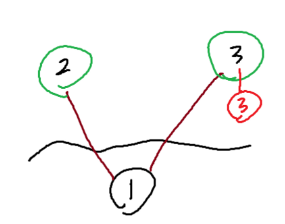
\includegraphics[bb=0 0 100 200]{1img.png}

\end{center} 
최초 트리의 형태이다. 첫 번째 쿼리시 1번을 흔들면 2, 3번 정점이 같이 흔들리고 3번 정점에 달린 열매를 떨어트리기 위해 3의 힘으로 흔들어야 한다.

\begin{center}

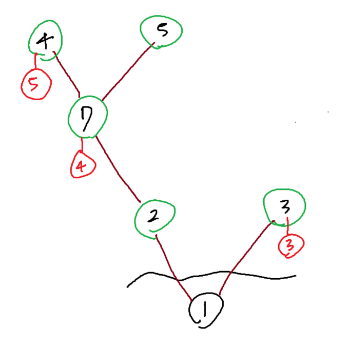
\includegraphics[bb=0 0 100 200]{2img.png}

\end{center} 
3개 접목을 진행한 모습이다. 4번을 흔들면 4번만 흔들리고, 4번에 달린 열매를 떨어트리기 위해 5의 힘으로 흔들어야 한다.
마찬가지로 7번을 흔들면 7, 4, 5번이 흔들리고 4번과 7번의 열매를 떨어트리기 위해 9의 힘으로 흔들어야 한다.

2번 예제를 봐보자
\begin{center}

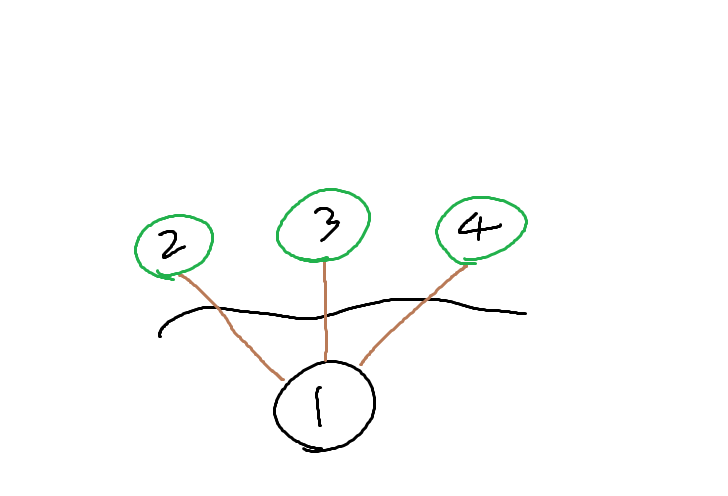
\includegraphics[scale=0.5]{3img.png}

\end{center} 
최초 트리의 형태이다. 첫 번째 쿼리시 1번을 흔들면 2, 3, 4번이 같이 흔들리지만, 열매가 달려있지 않다. 흔들어야 할 힘이 0이기에 -1을 출력한다.
\begin{center}

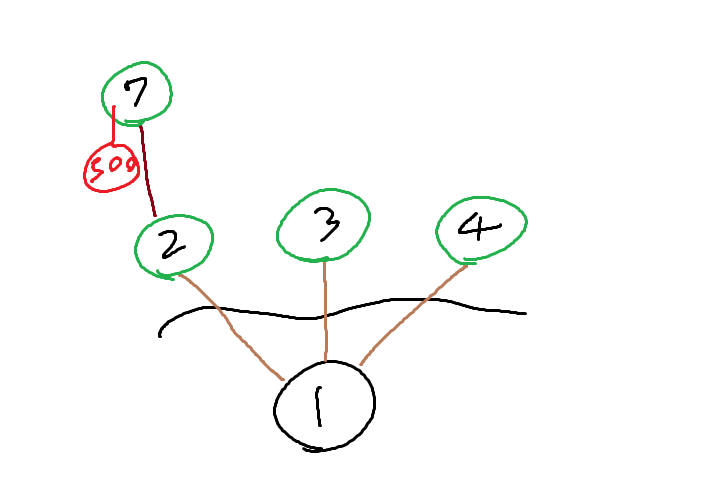
\includegraphics[scale=0.5]{4img.png}

\end{center} 
1개 접목을 진행한 모습이다. 1번을 흔들면 2, 3, 4, 7번이 같이 흔들리고, 7번의 열매를 떨어트리기 위해 500의 힘으로 흔들어야 한다.

\end{problem}

